\subsection{Encapsulation}
\textit{Apply encapsulation principles to a class -- Show an example of good encapsulation.  Show a bad example of encapsulation and explain why.  Additionally explain access modifiers and how they can be used as part of the class encapsulation.}

In the object-oriented paradigm, each object should be an independent unit of data and methods. The object should control how the data is accessed or manipulated. One object should not manipulate another object's data. This principle is called encapsulation.

It is achieved by marking all data fields private. Access to the fields is provided through getters and setters. These are methods that control how the fields are modified. 

For example, a class might have a field for a datetime. For calculation purposes, it is stored as a \texttt{long}, in Unix time\footnote{Seconds from 00:00:00 (UTC), Thursday, 1 January 1970. See \url{https://en.wikipedia.org/wiki/Unix_time}}. See figure \ref{fig:encapsulation} on page \pageref{fig:encapsulation} for a UML diagram of \texttt{EcapsulatedClass}. To make it easier to use the class, though, we provide a getter that returns the date as a \texttt{Date} object or formatted \texttt{String}. The getter takes the Unix time (\texttt{long}) and converts it to the \texttt{Date} or \texttt{String} object. We also provide a setter that takes in a \texttt{Date} or \texttt{Calendar} object, or a formatted \texttt{String}. We then convert it into a Unix time and store it in the \texttt{long} field. 

The user doesn't have to know how we store the data. We could change the internal workings of the class and the user wouldn't notice a thing. For example, we could start using two \texttt{long} fields, one for date, another for time. See the modified class, \texttt{EcapsulatedClass2} in figure \ref{fig:encapsulation} on page \pageref{fig:encapsulation}.

Failing to protect the data in this way is called the "Improper Intimacy" code smell\cite{codesmells}.

\begin{figure}[!h]\centering % Using \begin{figure*} makes the figure take up the entire width of the page
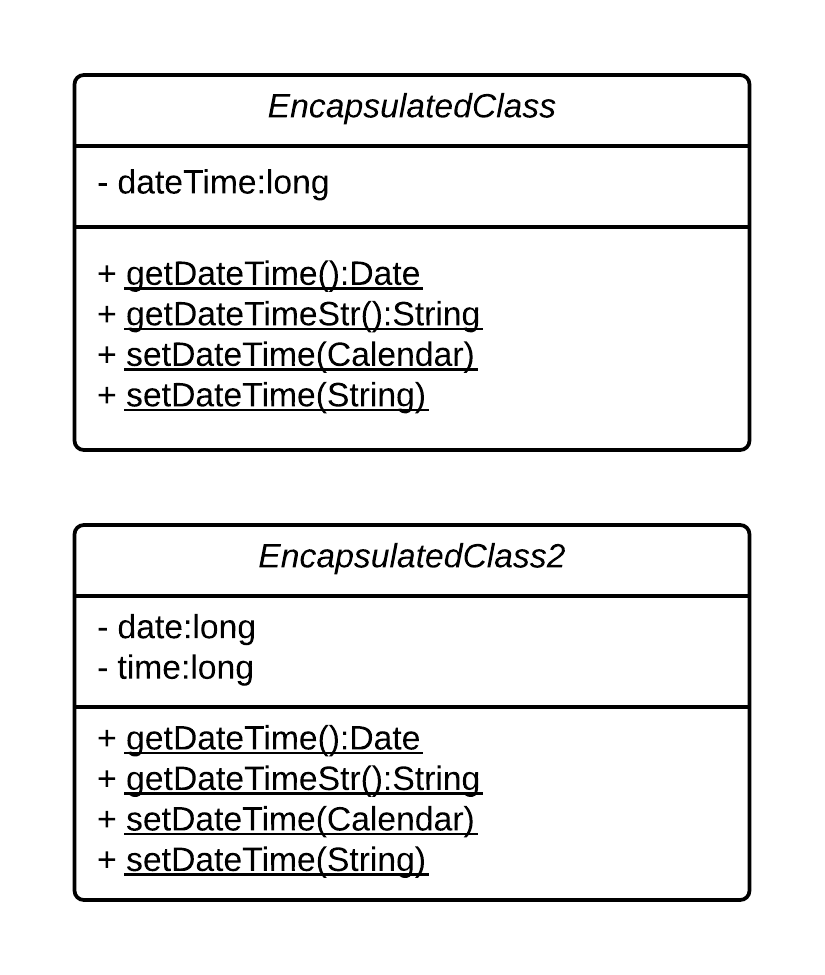
\includegraphics[width=0.9\linewidth, frame]{images/encapsulation}
\caption{Encapsulation}
\label{fig:encapsulation}
\end{figure}
"Feature Envy" code smell can be more subtle. It occurs when a method in a class makes too many calls to another class. Maybe the method really belongs to the class that is being called\cite{codesmells}. One class is doing too much of the work of another.For example, a \texttt{Dog} should not format the output of the \texttt{Tail} class. Instead, we define a \texttt{toString()} method in \texttt{Tail} and call that.

Encapsulation reduces bugs by giving each class a clear purpose. It also adds clarity to the code.
